%% ch_algorithms.tex — Algorithm Design
\chapter{ALGORITHM DESIGN}

This chapter presents the six core algorithms that constitute the Agentic Orchestrator. Each algorithm is formally defined with pseudocode, input/output specifications, and complexity analysis.

\section{Orchestrator Design Diagrams}

Figure~\ref{fig:rule_based} shows the Rule-Based Workflow.

\begin{figure}[H]
\centering
\begin{tikzpicture}[
  box/.style={draw, rounded corners, thick, minimum width=2.5cm, minimum height=0.8cm, align=center, fill=gray!10},
  arrow/.style={-latex, thick}
]
\node[box] (metrics) {Metrics};
\node[box, below=0.6cm of metrics] (thresh) {Threshold Check};
\node[box, below=0.6cm of thresh, fill=red!10] (cond) {RTT > SLA ?};
\node[box, below=0.6cm of cond, fill=orange!10] (throttle) {Throttle};
\node[box, below=0.6cm of throttle, fill=green!10] (restore) {Restore};

\draw[arrow] (metrics) -- (thresh);
\draw[arrow] (thresh) -- (cond);
\draw[arrow] (cond) -- node[right]{Yes} (throttle);
\draw[arrow] (throttle) -- (restore);
\draw[arrow] (cond.west) -- +(-1.5,0) |- node[left, pos=0.25]{No} (metrics.west);
\end{tikzpicture}
\caption{Rule-Based Workflow.}
\label{fig:rule_based}
\end{figure}

Figure~\ref{fig:agentic_flow} presents the Agentic Workflow.

\begin{figure}[H]
\centering
\begin{tikzpicture}[
  box/.style={draw, rounded corners, thick, minimum width=3.5cm, minimum height=0.8cm, align=center, fill=blue!10},
  arrow/.style={-latex, thick}
]
\node[box] (mon) {Monitoring Agent};
\node[box, below=0.5cm of mon] (state) {State Agent};
\node[box, below=0.5cm of state] (mem) {Memory Retrieval};
\node[box, below=0.5cm of mem, fill=purple!10] (llm) {LLM Planning Agent};
\node[box, below=0.5cm of llm] (val) {Validation Layer};
\node[box, below=0.5cm of val, fill=orange!10] (exec) {Execution Agent};
\node[box, below=0.5cm of exec] (memup) {Memory Update};

\draw[arrow] (mon) -- (state);
\draw[arrow] (state) -- (mem);
\draw[arrow] (mem) -- (llm);
\draw[arrow] (llm) -- (val);
\draw[arrow] (val) -- (exec);
\draw[arrow] (exec) -- (memup);
\end{tikzpicture}
\caption{Agentic Workflow.}
\label{fig:agentic_flow}
\end{figure}

Figure~\ref{fig:c345_framework} illustrates the integration of the C3, C4, and C5 frameworks.

\begin{figure}[H]
\centering
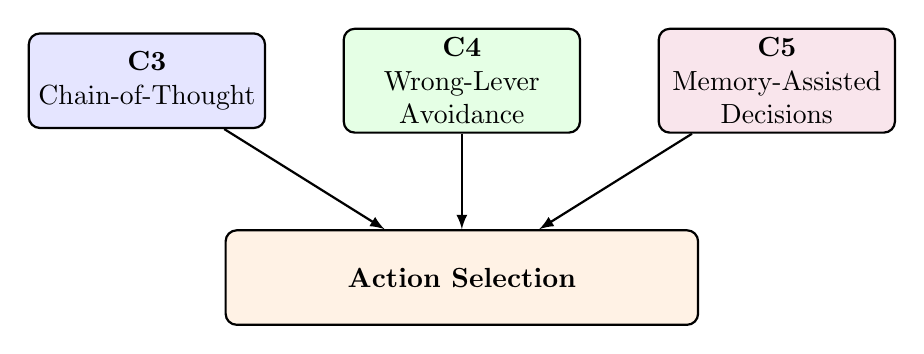
\begin{tikzpicture}[
  box/.style={draw, rounded corners, thick, minimum width=3cm, minimum height=1.2cm, align=center, fill=gray!10},
  arrow/.style={-latex, thick}
]
\node[box, fill=blue!10] (c3) at (0,2) {\textbf{C3}\\Chain-of-Thought};
\node[box, fill=green!10] (c4) at (4,2) {\textbf{C4}\\Wrong-Lever\\Avoidance};
\node[box, fill=purple!10] (c5) at (8,2) {\textbf{C5}\\Memory-Assisted\\Decisions};
\node[box, fill=orange!10, minimum width=6cm] (action) at (4,-0.5) {\textbf{Action Selection}};

\draw[arrow] (c3) -- (action);
\draw[arrow] (c4) -- (action);
\draw[arrow] (c5) -- (action);
\end{tikzpicture}
\caption{C3/C4/C5 Framework contributing to action selection.}
\label{fig:c345_framework}
\end{figure}

%% ─────────────────────────────────────────────────────────────
\section{Algorithm 1: Monitoring and State Collection}

Algorithm~\ref{alg:monitor} describes the decoupled monitoring thread that runs at a fixed 3-second interval independent of LLM inference.

\begin{algorithm}[H]
\caption{Monitoring Agent: Decoupled State Collection}
\label{alg:monitor}
\begin{algorithmic}[1]
\Require Monitoring interval $\Delta = 3\,\text{s}$, SSH credentials, Prometheus endpoint
\Ensure Updated thread-safe state cache $\mathcal{S}$

\While{orchestrator active}
  \State $t_0 \gets \text{time()}$

  \State \textbf{// Channel 1: URLLC RTT via SSH log parse}
  \State $R \gets \text{SSH.exec}(\texttt{"tail -1 /tmp/mec-clients/urllc-*.log"})$
  \State $R \gets \text{parseRTT}(R)$ \Comment{extract $\text{RTT}_{99}$ in ms}

  \State \textbf{// Channel 2: eMBB throughput from /proc/net/dev}
  \State $B_{\text{tx}}, B_{\text{rx}} \gets \text{readProcNetDev}(\texttt{uesimtun1})$
  \State $\lambda_{\text{bps}} \gets (B_{\text{tx}} - B_{\text{tx,prev}}) / \Delta \times 8$
  \State $\lambda_{\text{pkt}} \gets (\text{pkt}_{\text{tx}} - \text{pkt}_{\text{prev}}) / \Delta$

  \State \textbf{// Channel 3: mMTC PDR from MQTT log}
  \State $N_{\text{pub}}, N_{\text{ok}} \gets \text{parseMQTTLog}()$
  \State $\text{PDR} \gets N_{\text{ok}} / N_{\text{pub}}$ \textbf{ if } $N_{\text{pub}} > 0$ \textbf{ else } $1.0$

  \State \textbf{// Derived metrics}
  \State $\rho_{\text{eMBB}} \gets \text{computeLoadFraction}(\lambda_{\text{pkt}})$ \Comment{Algorithm~\ref{alg:loadfrac}}
  \State $d \gets \text{countDeadTunnels}()$

  \State \textbf{// Atomic state cache write}
  \State $\mathcal{S}.\text{acquire}()$
  \State $\mathcal{S} \gets \{R,\, \lambda_{\text{bps}},\, \lambda_{\text{pkt}},\, \rho_{\text{eMBB}},\, \text{PDR},\, d\}$
  \State $\mathcal{S}.\text{release}()$

  \State $\text{sleep}(\Delta - (\text{time}() - t_0))$
\EndWhile
\end{algorithmic}
\end{algorithm}

\textbf{Complexity:} $O(1)$ per cycle. SSH and file I/O dominate; total wall time $\approx 200$\,ms per cycle, leaving $\approx 2.8$\,s idle.

%% ─────────────────────────────────────────────────────────────
\section{Algorithm 2: eMBB Load Fraction Computation}

\begin{algorithm}[H]
\caption{eMBB Load Fraction with Sliding Window}
\label{alg:loadfrac}
\begin{algorithmic}[1]
\Require Packet rate $\lambda(t)$, window $W = 8$, history $\mathcal{H}$ (deque, maxlen $W$)
\Ensure $\rho_{\text{eMBB}}(t) \in [0,1]$ or \texttt{None}

\State $\mathcal{H}.\text{append}(\lambda(t))$
\If{$|\mathcal{H}| < \lceil W/2 \rceil$} \Comment{insufficient history}
  \Return \texttt{None}
\EndIf
\State $\lambda_{\max} \gets \max(\mathcal{H})$
\If{$\lambda_{\max} = 0$}
  \Return $0.0$ \Comment{slice is truly idle}
\EndIf
\Return $\lambda(t) / \lambda_{\max}$
\end{algorithmic}
\end{algorithm}

\textbf{Mathematical Formulation:} As defined in Eq.~\ref{eq:load_frac}, $\rho_{\text{eMBB}}$ normalises the current packet rate against the peak observed over the last $W$ cycles:
\[
  \rho_{\text{eMBB}}(t) = \frac{\lambda(t)}{\max_{k=0}^{W-1} \lambda(t - k\Delta)}
\]

\textbf{Why relative load is superior to absolute throughput:} An absolute threshold (e.g., throttle when eMBB $> 200$\,Mbps) will incorrectly trigger when the application itself is transmitting at 200\,Mbps by design. The relative metric is invariant to application-layer traffic profiles; only genuine burst anomalies ($\rho > 0.9$) drive orchestration decisions.

\textbf{Example:} $\mathcal{H} = [50, 120, 180, 220, 210, 190, 200, 215]$\,pkt/s, $\lambda(t) = 215$. Then $\lambda_{\max} = 220$, $\rho = 215/220 = 0.977$ — \textit{high load}: throttling is warranted.

\textbf{Sliding Window Complexity:} $O(W)$ per cycle for $\max$; $O(1)$ deque append.

%% ─────────────────────────────────────────────────────────────
\section{Algorithm 3: Agentic Planning (Chain-of-Thought)}

\begin{algorithm}[H]
\caption{Planning Agent: CoT-Enforced Action Selection}
\label{alg:plan}
\begin{algorithmic}[1]
\Require State $\mathcal{S}$, Agent Memory $\mathcal{M}$ (last $K=10$ entries)
\Ensure $\{\text{root\_cause},\, \text{lever\_validity},\, \text{action},\, r',\, c\}$

\State $\pi \gets \text{buildSystemPrompt}()$ \Comment{forbids thresholds, mandates CoT schema}
\State $\mu \gets \text{summariseMemory}(\mathcal{M})$ \Comment{last $K$ (action, $\Delta R$) pairs}
\State $\sigma \gets \text{formatStateVector}(\mathcal{S})$ \Comment{RTT, $\rho$, trend, stable\_for, \ldots}
\State $\text{prompt} \gets \pi \oplus \sigma \oplus \mu$

\State $\text{raw} \gets \text{LLM.generate}(\text{prompt},\, \texttt{format=json},\, \texttt{timeout}=60)$

\If{$\text{raw} = \emptyset$} \Comment{timeout}
  \Return $\text{RuleBasedFallback}(\mathcal{S})$ \Comment{Algorithm~\ref{alg:loop}}
\EndIf

\State $\text{cot} \gets \text{parseJSON}(\text{raw})$
\State \textbf{assert} \texttt{root\_cause} $\neq \emptyset$ \textbf{ and } \texttt{lever\_validity} $\neq \emptyset$
\State $r' \gets \text{int}(\text{cot.new\_rate\_mbit})$ \textbf{ or } $r_{\max}$
\State $c \gets \text{float}(\text{cot.confidence})$

\Return $\{\text{cot.root\_cause},\, \text{cot.lever\_validity},\, \text{cot.action},\, r',\, c\}$
\end{algorithmic}
\end{algorithm}

%% ─────────────────────────────────────────────────────────────
\section{Algorithm 4: Validation and Safety Gate}

\begin{algorithm}[H]
\caption{Validation Gate: Safety and Contradiction Detection}
\label{alg:validate}
\begin{algorithmic}[1]
\Require CoT output $\{a, r', c, \text{root\_cause}\}$, bounds $[r_{\min}, r_{\max}]$
\Ensure Safe action $a^*$, adjusted confidence $c^*$

\State \textbf{// Range clamp}
\State $r^* \gets \max(r_{\min},\, \min(r', r_{\max}))$

\State \textbf{// Contradiction detection (Contribution C4)}
\State $\mathcal{K} \gets \{$\textit{"low load", "not the cause", "nearly idle", "not embb"}$\}$
\If{$a = \texttt{throttle\_embb}$ \textbf{ and } $\exists k \in \mathcal{K} : k \in \text{root\_cause}$}
  \State $c^* \gets 0.5 \times c$ \Comment{penalise contradictory reasoning}
  \State $\log.\text{warning}(\texttt{"Contradiction detected"})$
\Else
  \State $c^* \gets c$
\EndIf

\State \textbf{// Dead-tunnel guard}
\If{$\mathcal{S}.\text{dead\_tunnels} = 3$} \Comment{all URLLC tunnels dead}
  \Return $\{\texttt{no\_action},\, r_{\max},\, 0.0\}$ \Comment{monitoring unreliable}
\EndIf

\State \textbf{// Redundant-action guard}
\If{$a = \texttt{throttle\_embb}$ \textbf{ and } $r^* = r_{\text{current}}$}
  \Return $\{\texttt{no\_action},\, r_{\text{current}},\, c^*\}$
\EndIf

\Return $\{a,\, r^*,\, c^*\}$
\end{algorithmic}
\end{algorithm}

%% ─────────────────────────────────────────────────────────────
\section{Algorithm 5: Memory Update and Retention}

\begin{algorithm}[H]
\caption{Agent Memory: Update and Context Summarisation}
\label{alg:memory}
\begin{algorithmic}[1]
\Require Action $a$, pre-action state $\mathcal{S}_{\text{pre}}$, post-action RTT $R_{\text{post}}$, Memory $\mathcal{M}$ (deque, maxlen $K=10$)
\Ensure Updated $\mathcal{M}$ with outcome

\State $\Delta R \gets R_{\text{post}} - \mathcal{S}_{\text{pre}}.\text{RTT}$ \Comment{outcome delta}
\State $\text{outcome} \gets$ \textbf{if} $\Delta R < -2$: \texttt{"improved"} \textbf{elif} $\Delta R > 2$: \texttt{"worsened"} \textbf{else}: \texttt{"neutral"}

\State $e \gets \{\text{ts},\, a,\, \mathcal{S}_{\text{pre}}.\rho,\, \mathcal{S}_{\text{pre}}.\text{RTT},\, R_{\text{post}},\, \Delta R,\, \text{outcome}\}$
\State $\mathcal{M}.\text{append}(e)$ \Comment{oldest entry evicted if full}

\State \textbf{// Context summary for next LLM prompt}
\State $\text{summary} \gets \emptyset$
\ForAll{$e_i \in \mathcal{M}$}
  \State $\text{summary} \gets \text{summary} + \texttt{"[}\,e_i.\text{ts}\,\texttt{]}\,a_i:\,\rho=\,\rho_i,\,\Delta R=\,\Delta R_i\,(\text{outcome}_i)"$
\EndFor
\Return $\mathcal{M}$, $\text{summary}$
\end{algorithmic}
\end{algorithm}

\textbf{Retention Policy:} The ring buffer of depth $K = 10$ ensures $O(1)$ insertion. Only the $K$ most recent decisions are injected into the LLM prompt, capping context token overhead at approximately 400 tokens regardless of session length.

%% ─────────────────────────────────────────────────────────────
\section{Algorithm 6: Autonomous Control Loop}

Algorithm~\ref{alg:loop} presents the complete closed-loop orchestration workflow integrating all five agents.

\begin{algorithm}[H]
\caption{Autonomous Closed-Loop Orchestration}
\label{alg:loop}
\begin{algorithmic}[1]
\Require SLA threshold $\theta$, rate bounds $[r_{\min}, r_{\max}]$, LLM endpoint
\Ensure Continuous QoS enforcement across eMBB, URLLC, mMTC slices

\State Initialise state $\mathcal{S} \gets \{\}$, Memory $\mathcal{M} \gets \emptyset$, $r_{\text{current}} \gets r_{\max}$
\State \textbf{spawn} MonitoringThread (Algorithm~\ref{alg:monitor}) \Comment{decoupled, 3-second loop}
\State Initialise HTB qdisc on worker node (Section 4.3)

\Loop \Comment{main orchestration cycle}
  \State \textbf{// Observe}
  \State $\mathcal{S} \gets \mathcal{S}.\text{snapshot}()$ \Comment{read from thread-safe cache}
  \State $\mathcal{S} \gets \text{StateAgent.update}(\mathcal{S})$ \Comment{trend, violation\_count}

  \State \textbf{// Think}
  \State $\{a, r', c, \ldots\} \gets \text{PlanningAgent}(\mathcal{S}, \mathcal{M})$ \Comment{Algorithm~\ref{alg:plan}}

  \State \textbf{// Validate}
  \State $\{a^*, r^*, c^*\} \gets \text{ValidationGate}(a, r', c, \mathcal{S})$ \Comment{Algorithm~\ref{alg:validate}}

  \If{$c^* \geq 0.5$ \textbf{ or } LLM timed out}
    \State \textbf{// Act}
    \State $\mathcal{S}_{\text{pre}} \gets \mathcal{S}$
    \State $\text{ExecutionAgent.run}(a^*, r^*)$ \Comment{SSH \texttt{tc class change}}
    \State $r_{\text{current}} \gets r^*$
    \State $\text{StateAgent.record\_action}(a^*, r^*)$

    \State \textbf{// Reflect: wait one monitoring cycle, capture outcome}
    \State $\text{sleep}(3)$
    \State $R_{\text{post}} \gets \mathcal{S}.\text{snapshot}().\text{RTT}$
    \State $\mathcal{M} \gets \text{MemoryAgent.update}(a^*, \mathcal{S}_{\text{pre}}, R_{\text{post}}, \mathcal{M})$ \Comment{Algorithm~\ref{alg:memory}}
  \EndIf

  \State \textbf{// Expose metrics}
  \State $\text{Prometheus.export}(\mathcal{S}, r_{\text{current}}, \mathcal{M})$
\EndLoop
\end{algorithmic}
\end{algorithm}

\textbf{Complexity:} The dominant cost is LLM inference at $O(T_{\text{llm}}) \approx 25$--$30$\,s. The monitoring thread runs at $O(1)$ per 3-second cycle. The total system overhead on the master node is approximately 62\% CPU utilisation during inference.
